% Created 2015-10-29 Thu 23:42
\documentclass{article}
\usepackage[top=1in, bottom=1.in, left=1in, right=1in]{geometry}
  \usepackage[makeroom]{cancel}
\usepackage{verbatim}


\usepackage[utf8]{inputenc}
\usepackage{lmodern}
\usepackage[T1]{fontenc}
\usepackage{fixltx2e}
\usepackage{graphicx}
\usepackage{longtable}
\usepackage{float}
\usepackage{wrapfig}
\usepackage{rotating}
\usepackage[normalem]{ulem}
\usepackage{amsmath}
\usepackage{textcomp}
\usepackage{marvosym}
\usepackage{wasysym}
\usepackage{amssymb}
\usepackage{amsmath}
\usepackage[version=3]{mhchem}
\usepackage[numbers,super,sort&compress]{natbib}
\usepackage{natmove}
\usepackage{url}
\usepackage{minted}
\usepackage{underscore}
\usepackage[linktocpage,pdfstartview=FitH,colorlinks,
linkcolor=blue,anchorcolor=blue,
citecolor=blue,filecolor=blue,menucolor=blue,urlcolor=blue]{hyperref}
\usepackage{attachfile}
\author{Abhishek Bagusetty}
\date{\today}
\title{24-623 2015 HM4}
\begin{document}

\maketitle

\section{Problem 1}
\label{sec-1}
The regular equations for the velocity verlet scheme are as follows: 

\begin{enumerate}
\item $v_{i}(t+\Delta t/2) = v_{i}(t) + F_{i}(t) \Delta t/2m_{i}$
\item $r_{i}(t+\Delta t) = r_{i}(t) + v_{i}(t+\Delta t/2)\Delta t$
\item $v_{i}(t+\Delta t) = v_{i}(t+\Delta t)+ F_{i}(t+\Delta t) \Delta t/2m_{i}$
\end{enumerate}

With MD simulations in NVT ensemble using the Nose-Hoover thermostat, the following are the equations of motions,

\begin{enumerate}
\item $\dot{r_{i}} = \mathbf{v_{i}}$
\item $\dot{\mathbf{v_{i}}} = \mathbf{F_{i}}/m_{i} - \eta \mathbf{v_{i}}$
\item $\eta = \frac{1}{\tau^2_{T}} \Big(\frac{T}{T_{set}} -1 \Big)$
\end{enumerate}

Now replacing the acceleration term with the above equations of motion.

\begin{equation}
  v_{i}(t+\Delta t/2) = v_{i}(t) + (\mathbf{F_{i}(t)/m_{i}}) \Delta t/2
  \label{eq:eq1}
\end{equation}

\begin{equation}
F_{i}(t)/m_{i} = a_{i} \implies \dot{\mathbf{v_{i}}} = \mathbf{F_{i}}/m_{i} - \eta \mathbf{v_{i}}
\end{equation}

Now substitute the above equation in original Step 3,
\begin{equation}
\boxed{ v_{i}(t+\Delta t/2) = v_{i}(t) + [\mathbf{F_{i}}/m_{i} - \eta(t) \mathbf{v_{i}(t)}] \Delta/2 }
\end{equation}

The Step 2 for the evolution of position remains the same as the actual expression.

The Step 3 is driven by the $F_{i}(t+\Delta t)/m_{i}$, which is the acceleration at $(t+\Delta t)$

\begin{equation}
  v_{i}(t+\Delta t) = v_{i}(t+\Delta t/2) + F_{i}(t+\Delta t) \Delta t/2m_{i}
  \label{eq:eq2}
\end{equation}
If we replace the force term at $(t+\Delta t)$ from the Step 3 with the modified equations of motions as follows,

\begin{equation}
\dot{\mathbf{v_{i}}}(t+\Delta t) = \mathbf{F_{i}(t+\Delta t)}/m_{i} - \eta(t+\Delta t) \mathbf{v_{i}(t+\Delta t)}
\end{equation}
Substitute the above expression in \ref{eq:eq2}, would give

\begin{equation}
  v_{i}(t+\Delta t) = v_{i}(t+\Delta t) + [\mathbf{F_{i}(t+\Delta t)}/m_{i} - \eta(t+\Delta t) \mathbf{v_{i}(t+\Delta t)}] \Delta t/2
  \label{eq:eq3}
\end{equation}

Rearranging the expression results in,

\begin{equation}
  v_{i}(t+\Delta t) = v_{i}(t+\Delta t) + F_{i}(t+\Delta t) \Delta t/(2m_{i}) - v_{i}(t+\Delta t) \eta(t+\Delta t)\Delta t/2
\end{equation}

\begin{equation}
  v_{i}(t+\Delta t)\Big(1 + \eta(t+\Delta t)\Delta t/2 \Big) = v_{i}(t+\Delta t) + F_{i}(t+\Delta t) \Delta t/(2m_{i})
\end{equation}

\begin{equation}
\boxed{ \mathbf{v}_{i}(t+\Delta t) = \frac{\mathbf{v}_{i}(t+\Delta t) + \mathbf{F}_{i}(t+\Delta t) \Delta/(2m_{i})}{1 + \eta(t+\Delta t)\Delta t/2} } 
\end{equation}

Note that the $\eta(t+\Delta t)$ is obtained from the modified equation of motion using simple forward difference rule:

\begin{equation}
\dot{\eta} = \frac{d\eta}{dt} = \frac{1}{\tau^2_{T}} \Big(\frac{T}{T_{set}} - 1\Big)
\end{equation}

\begin{equation}
\frac{\eta(t+\Delta t) - \eta(t)}{\Delta t} = \frac{1}{\tau^2_{T}} \Big(\frac{T}{T_{set}} - 1\Big) 
\end{equation}

\begin{equation}
\boxed{ \eta(t+\Delta t) = \eta(t) + \frac{\Delta t}{\tau^2_{T}} \Big(\frac{T}{T_{set}} - 1\Big) }
\end{equation}

\section{Problem 2}
\label{sec-2}
\subsection{a)}
\label{sec-2-1}

Average Pressure is plotted as the function of density between 950 $kg/m^3$ and 1150 $kg/m^3$. A trendline is fit and the zero pressure density is found to be at 1042.8 $kg/m^3$ which slightly varies with the density computed from the previous computations corresponding to 1053.8 $kg/m^3$.

\begin{enumerate}
\item Several NVT simulations are performed with NVT ensemble and Nose-Hoover thermostat and ensuring temperature of 100K is reached for every run.

\item Equlibration is completed, as judged by the lack of energy drift in the 200 units of MD simulation. $\big\langle (E-\langle E \rangle) \big\rangle$ per atom is in the order of 1e-3 which indicate the energy fluctuations are very small.
\end{enumerate}

Plots of energies, temeprature and pressure are shown below for a configuration approaching zero pressure NVT simulation for 200 LJ units. Plots for all other configurations can be found in the submission file. The plots are shown in Figs.\ref{fig:P2a1}, \ref{fig:P2a2}, \ref{fig:P2a3} respectively.

\begin{figure}[htb]
\centering
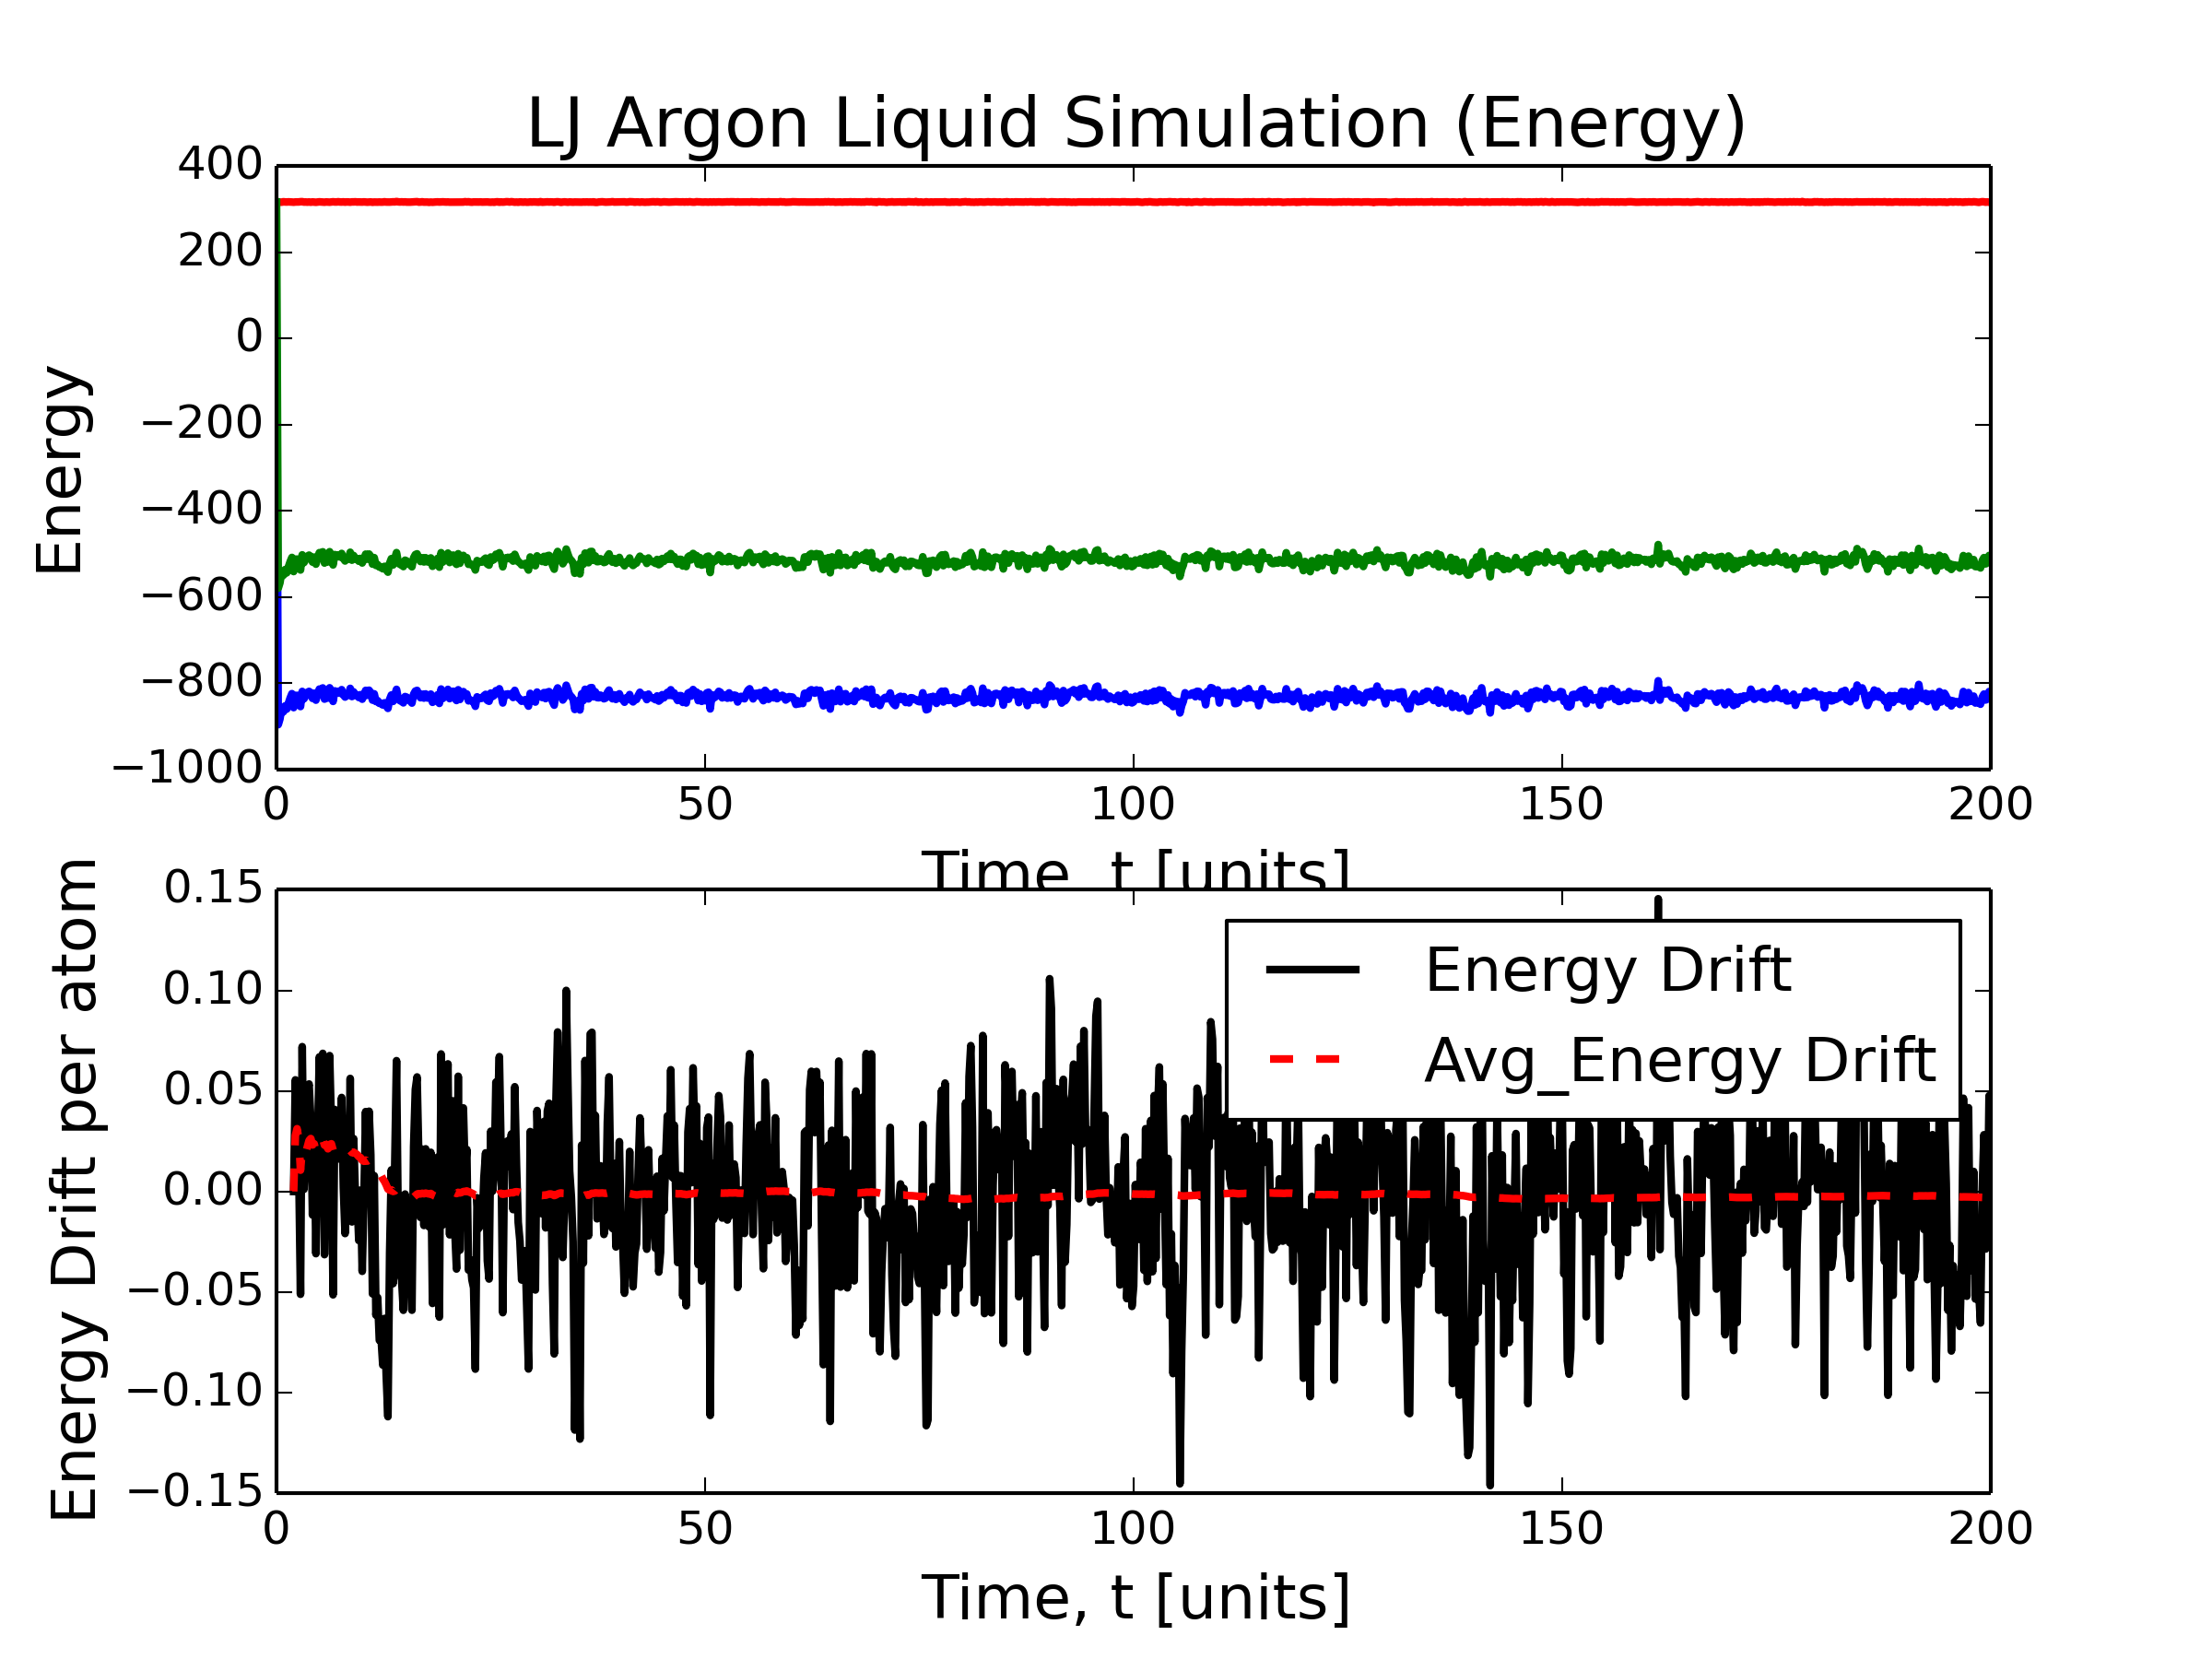
\includegraphics[width=.9\linewidth]{./V-4/LJ-md-Ener.png}
\caption{\label{fig:P2a1}The figure shows the time evolution of energy and energy drift showing the equilibration of the system}
\end{figure}

\begin{figure}[htb]
\centering
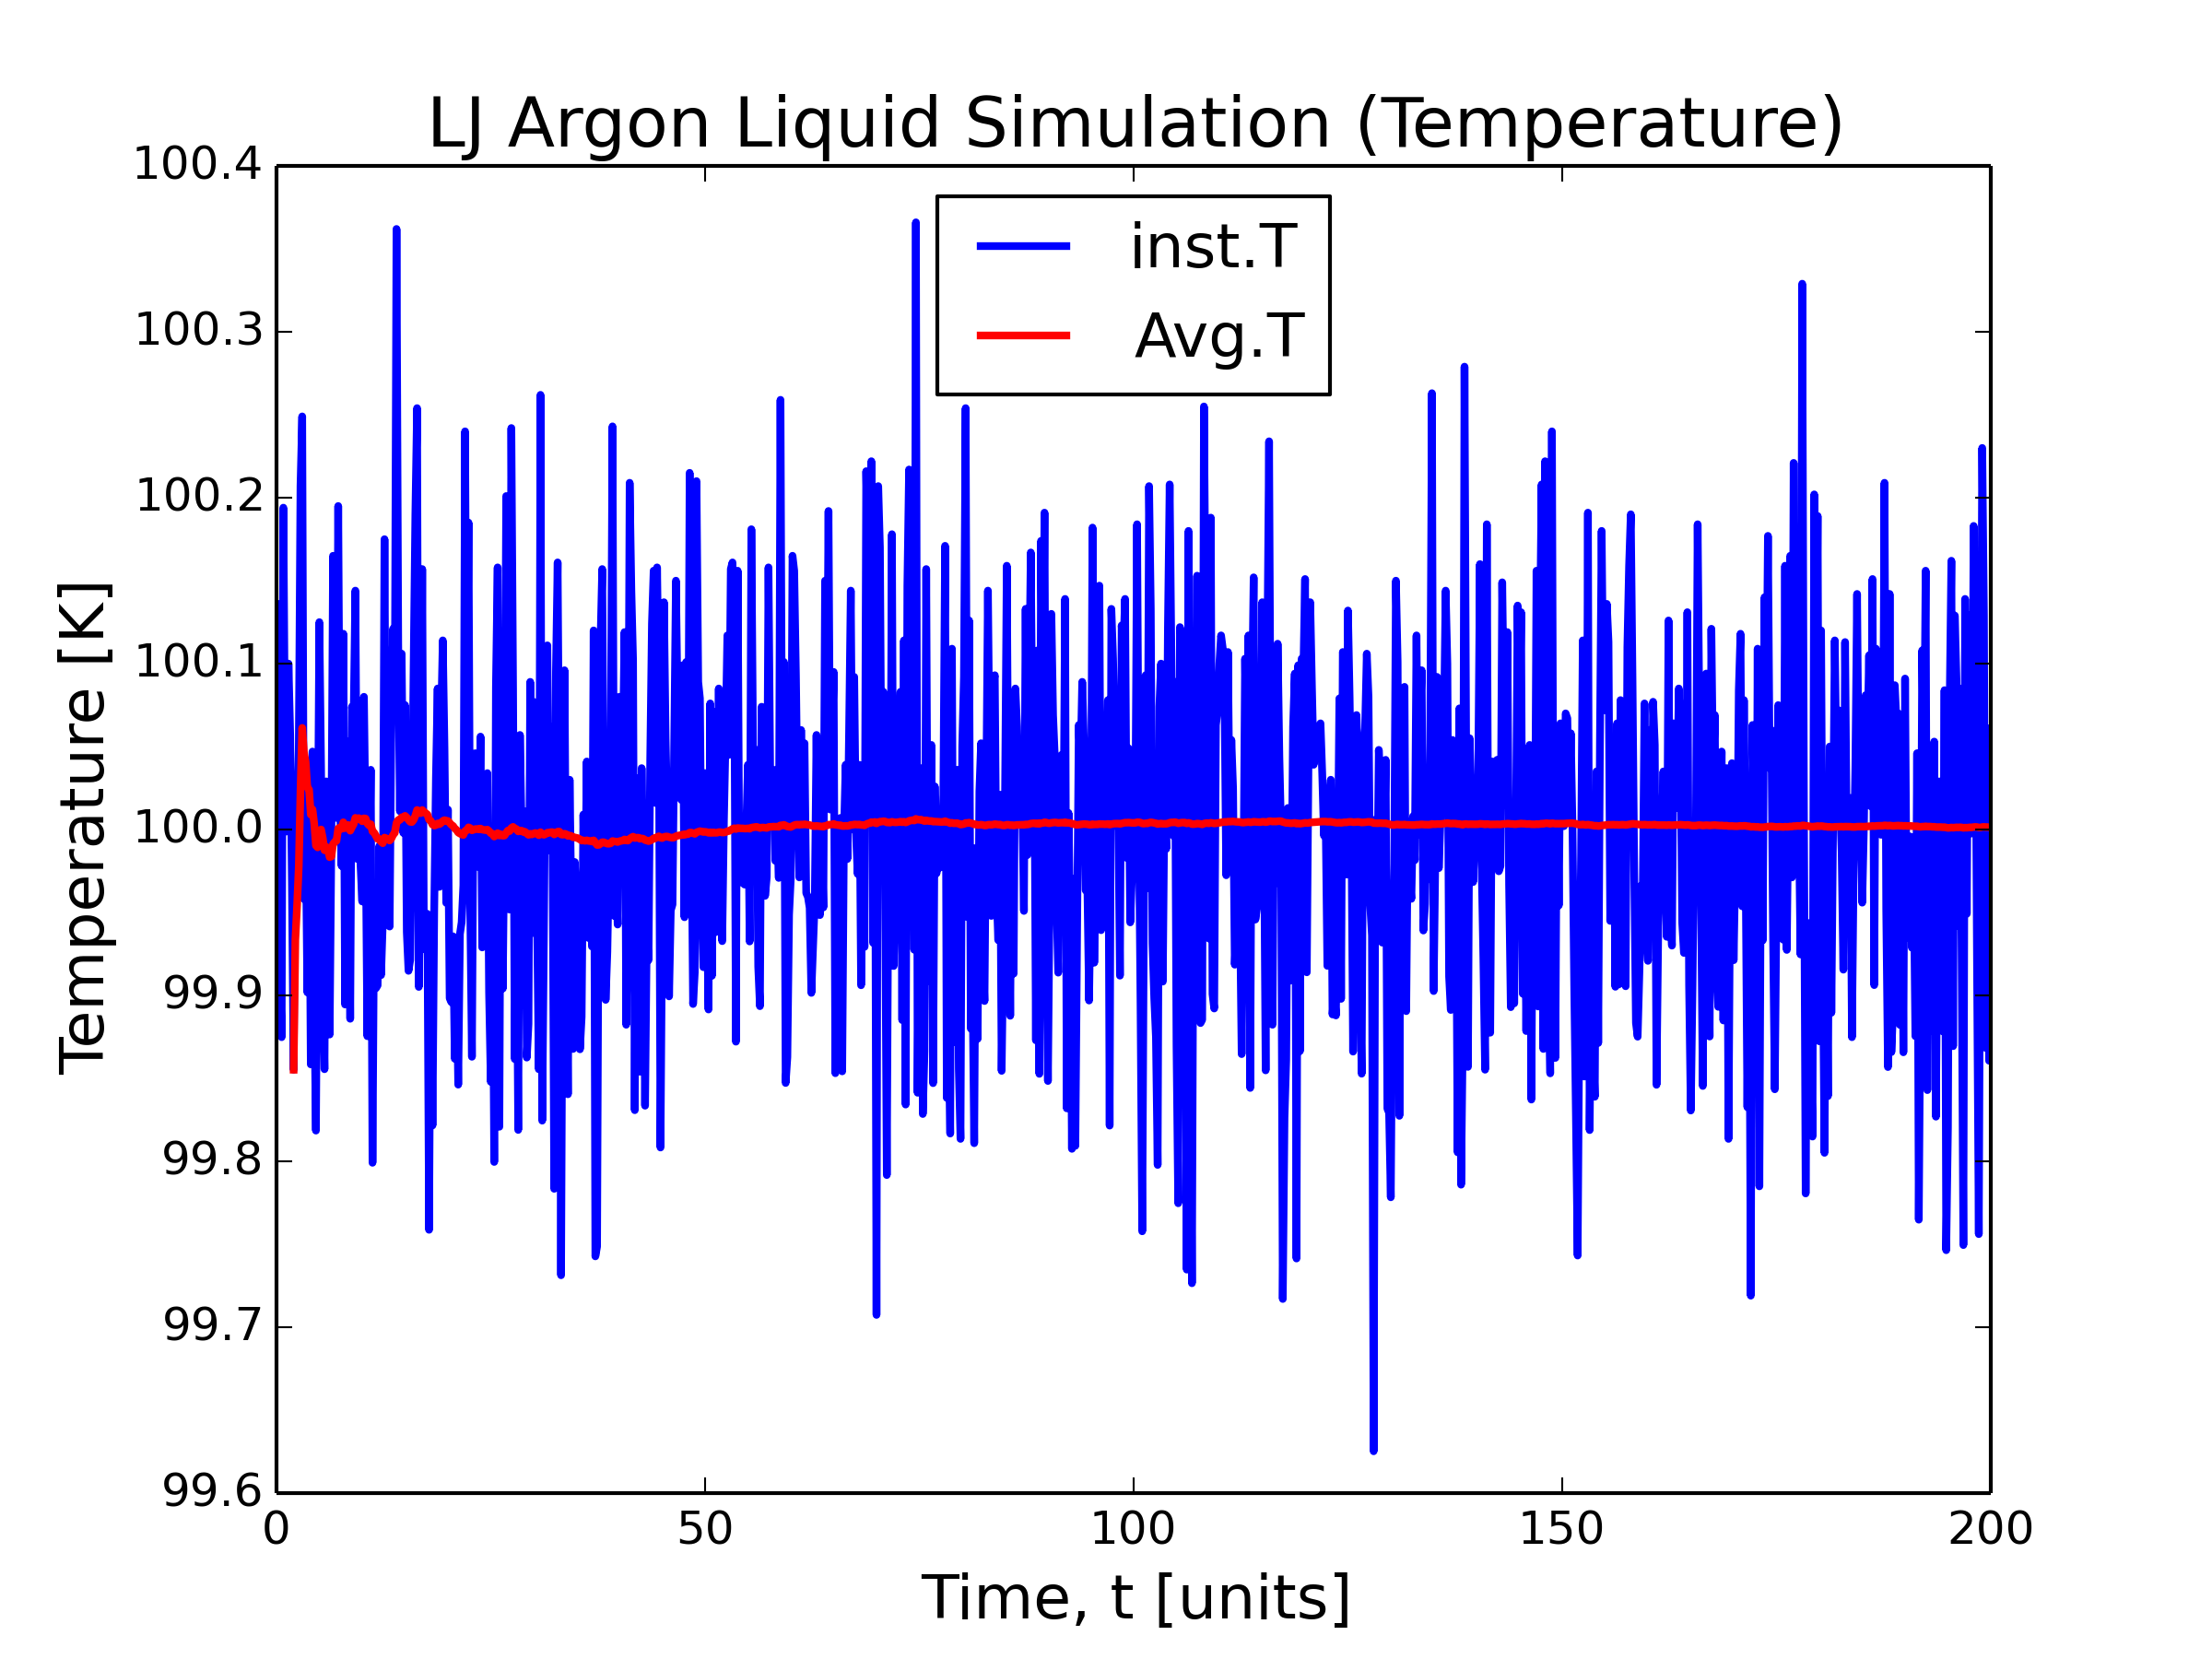
\includegraphics[width=.9\linewidth]{./V-4/LJ-md-Temp.png}
\caption{\label{fig:P2a2}The figure shows the time evolution of temeprature and the equilibration of average temperature to 100K.}
\end{figure}

\begin{figure}[htb]
\centering
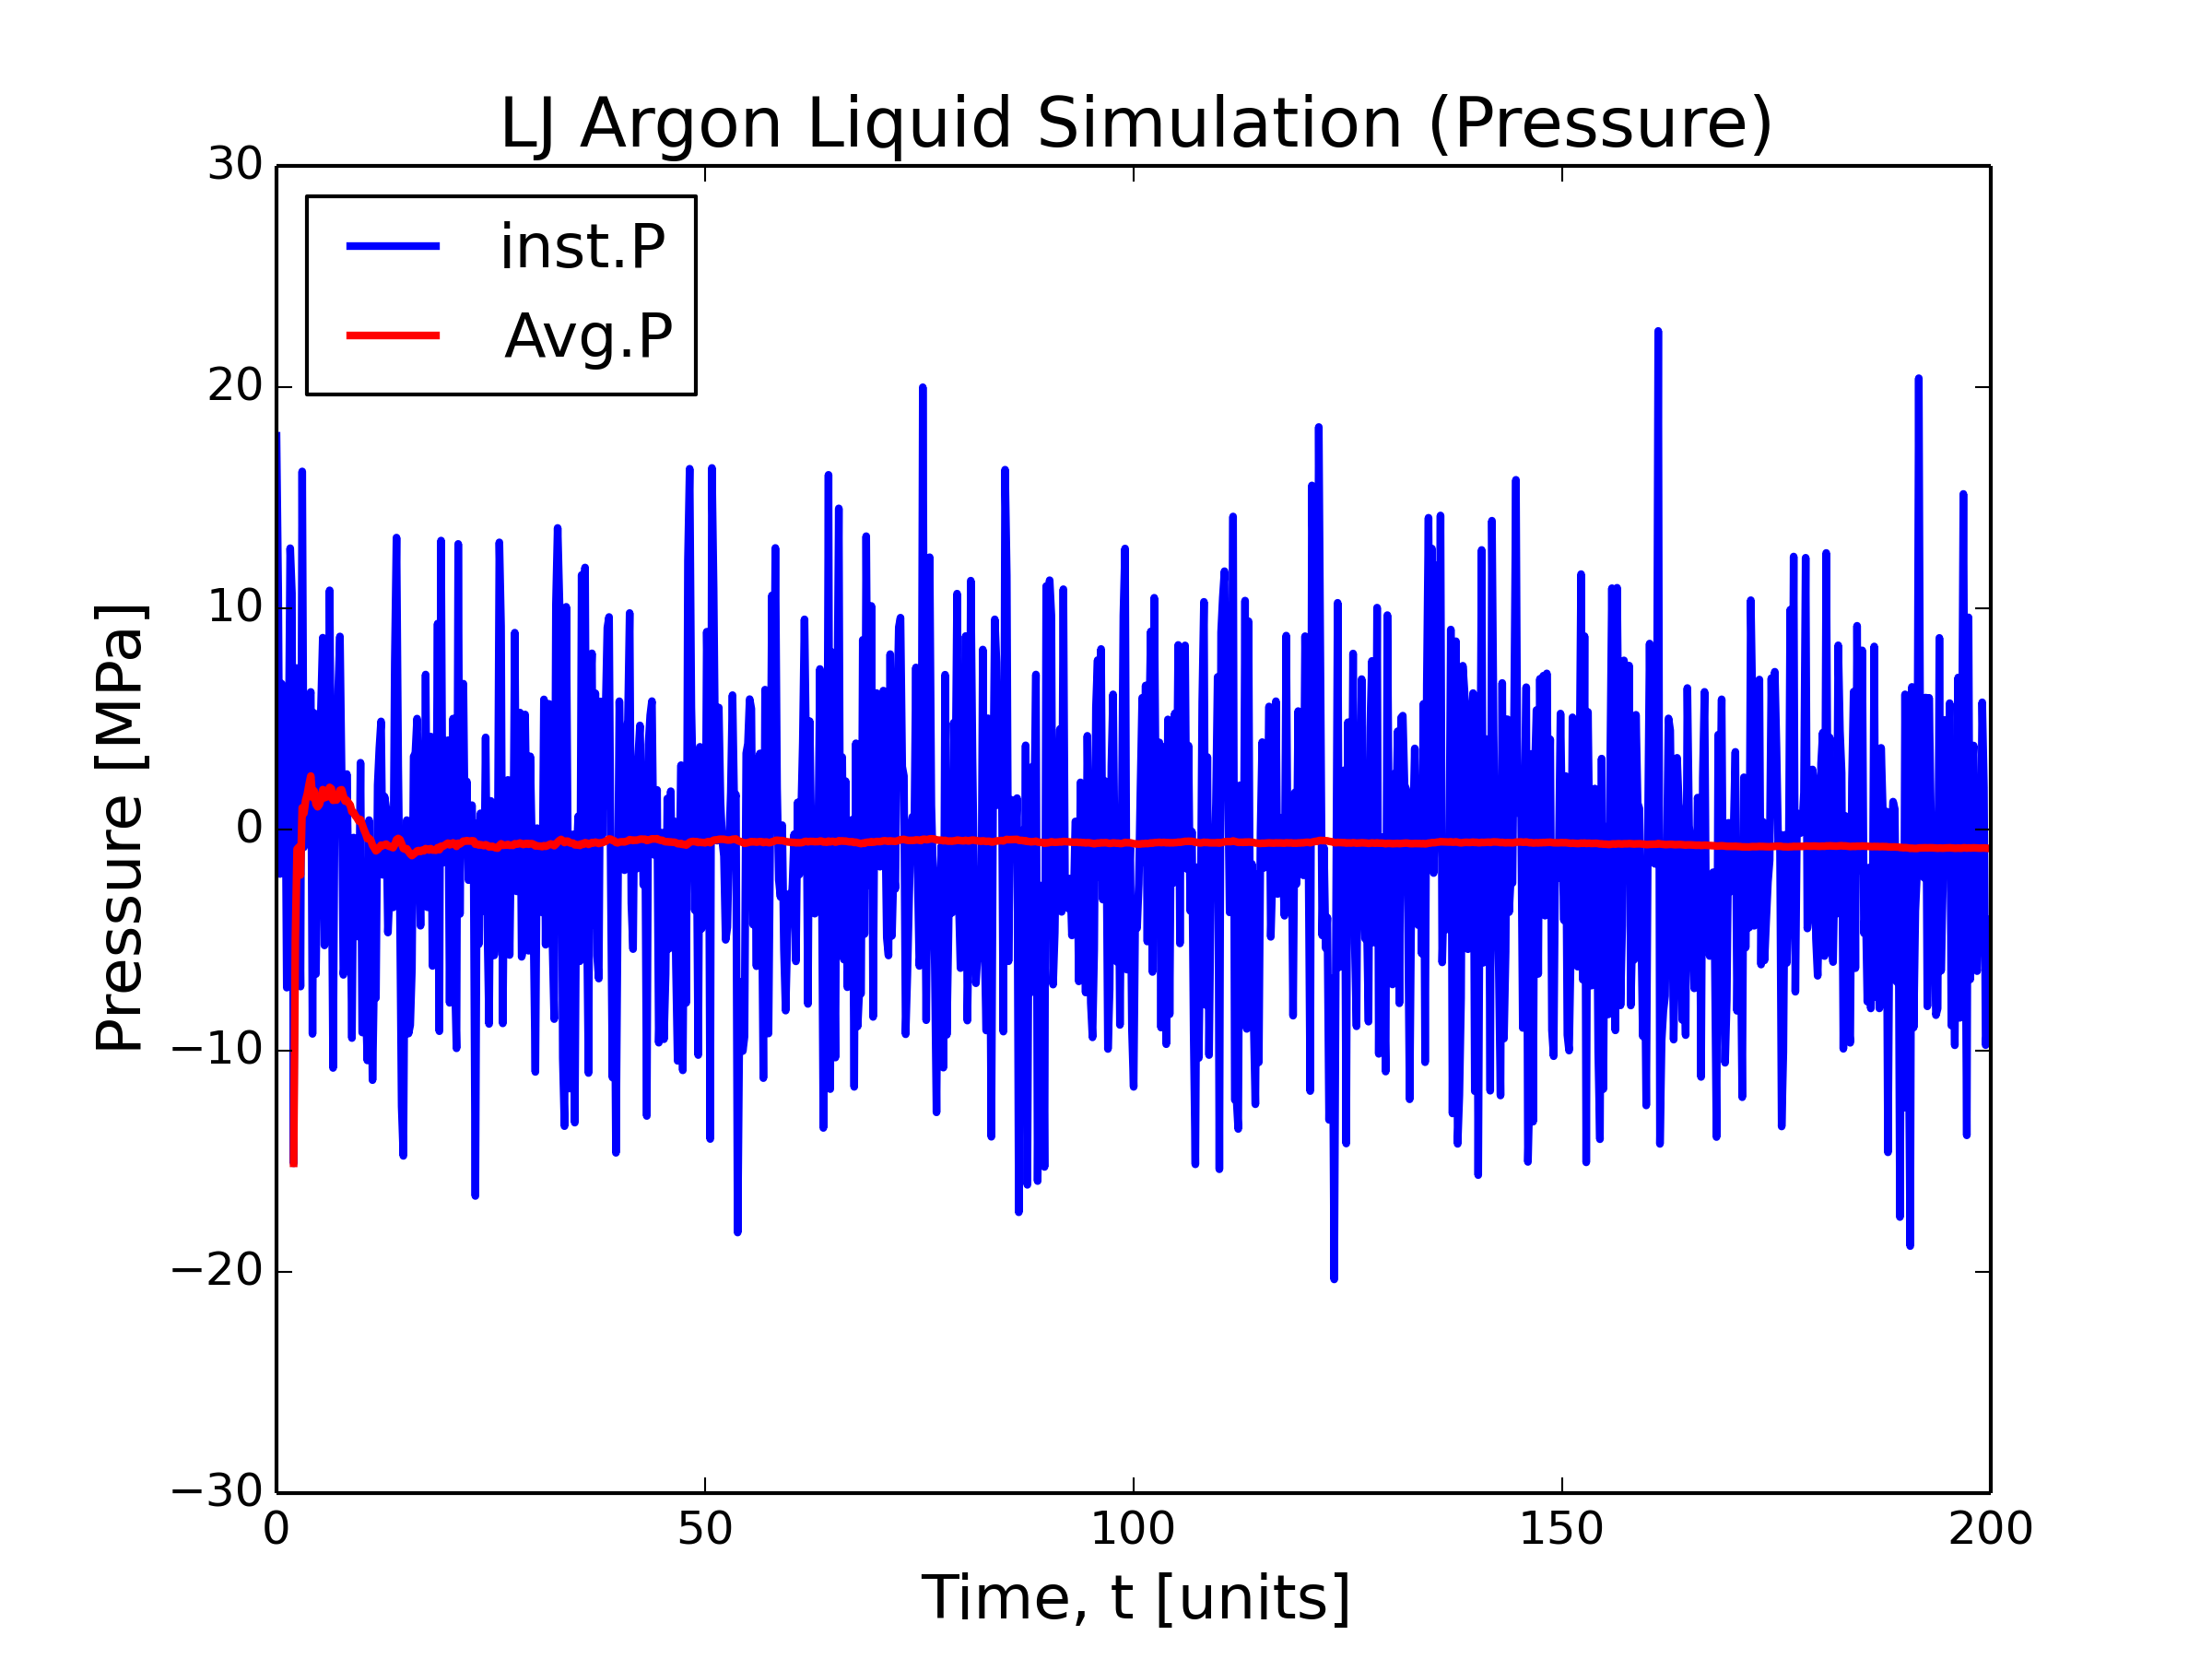
\includegraphics[width=.9\linewidth]{./V-4/LJ-md-Pressure.png}
\caption{\label{fig:P2a3}The figure shows the time evolution of Pressure and its closest approach to zero pressure.}
\end{figure}

Plot of average pressure in non-dimensional units is plotted against the density and a trendline is fit as shown below in Fig.\ref{fig:P2a}

\begin{figure}[htb]
\centering
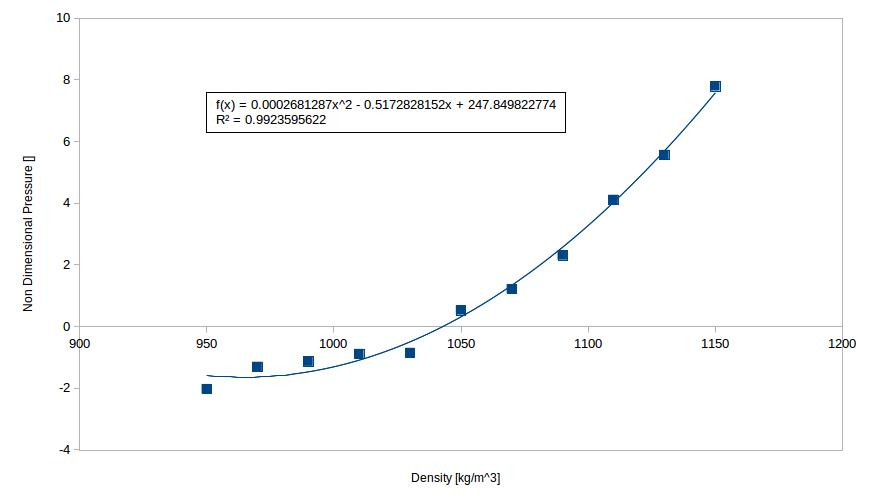
\includegraphics[width=.9\linewidth]{./HM4-P2a.jpg}
\caption{\label{fig:P2a}The figure shows the plot of average pressure as a function of density.}
\end{figure}



\section{Problem 3}
\label{sec-3}
% Emacs 24.5.1 (Org mode 8.2.10)
\end{document}